\chapter{Quick Start}

\begin{itemize}
\item Connect Picosafe with an usb cable to your pc
\item Two mass storages appears (one with an start.html and a public open flash disk)
\item Click on start.html 
\item Click on start link (to url https://172.24.42.1)
\item Acknowledge the self signes SSL certificate
\item With windows you have to first install the picosafe.inf (Please accept not trusted driver)
\item Open the decrypted filesystem with the default password: picosafe
\item After the stick is ready the main screen appears automatically (sometimes this needs some time)
\item Connect you with ssh to change the default passwords
\end{itemize}

\begin{wrapfigure}{r}{1.0\textwidth}
  \begin{center}
    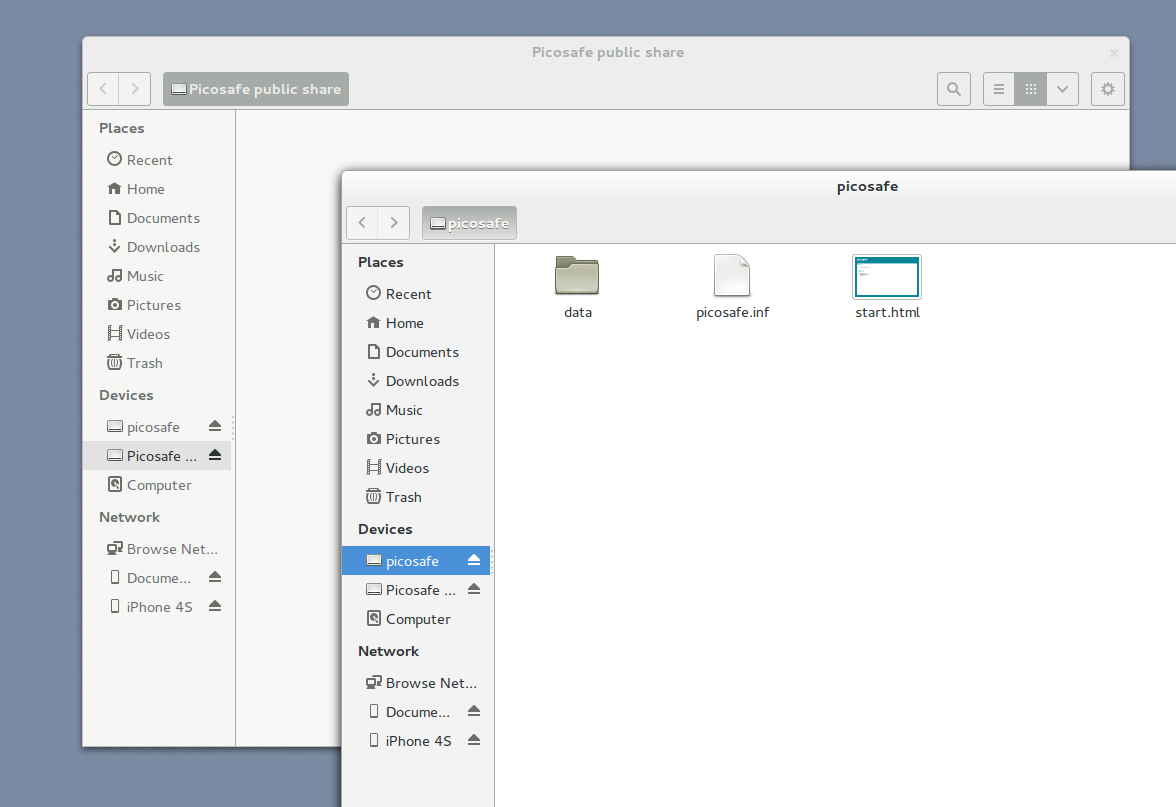
\includegraphics[width=0.70\textwidth]{picosafe_volumes_start.png}
  \end{center}
  \caption{Drives after connect Picosafe to USB.}
\end{wrapfigure}


\begin{wrapfigure}{r}{1.0\textwidth}
  \begin{center}
    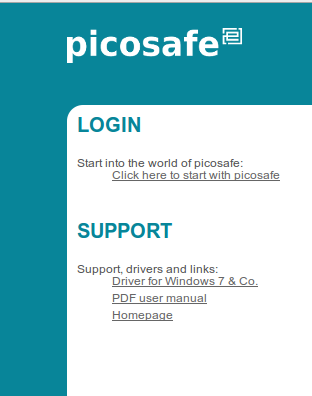
\includegraphics[width=0.70\textwidth]{picosafe_volumes_startlink.png}
  \end{center}
  \caption{Open start.html and click on start}
\end{wrapfigure}


\begin{wrapfigure}{r}{1.0\textwidth}
  \begin{center}
    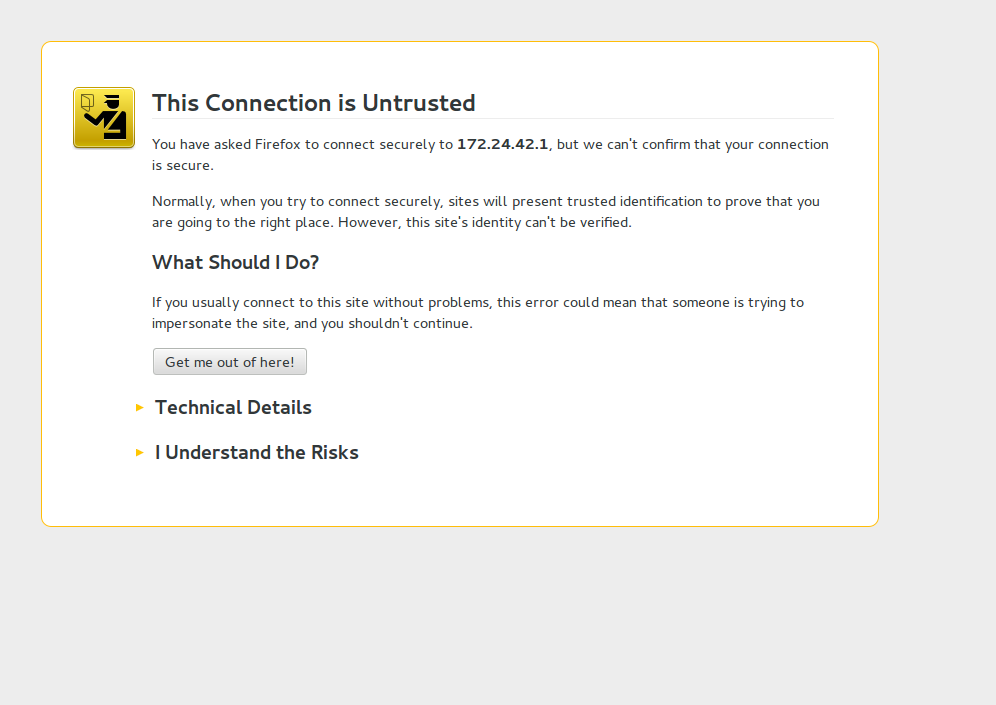
\includegraphics[width=0.70\textwidth]{ssl.png}
  \end{center}
  \caption{Click: I Understand the risk}
\end{wrapfigure}

\begin{wrapfigure}{r}{1.0\textwidth}
  \begin{center}
    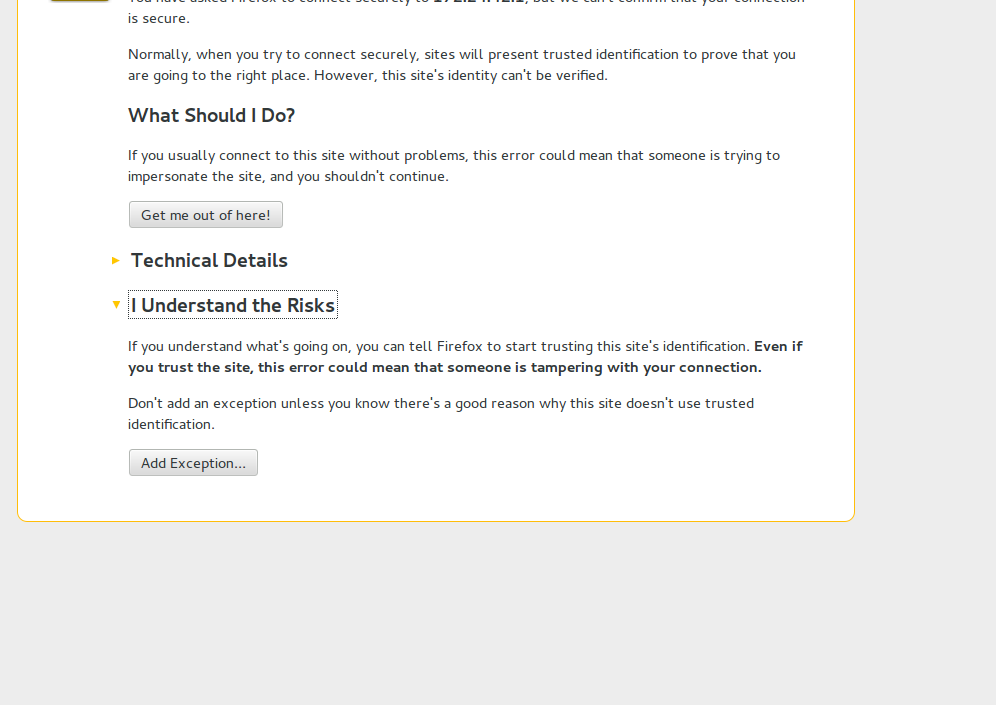
\includegraphics[width=0.70\textwidth]{ssl2.png}
  \end{center}
  \caption{Click: Add Exception}
\end{wrapfigure}

\begin{wrapfigure}{r}{1.0\textwidth}
  \begin{center}
    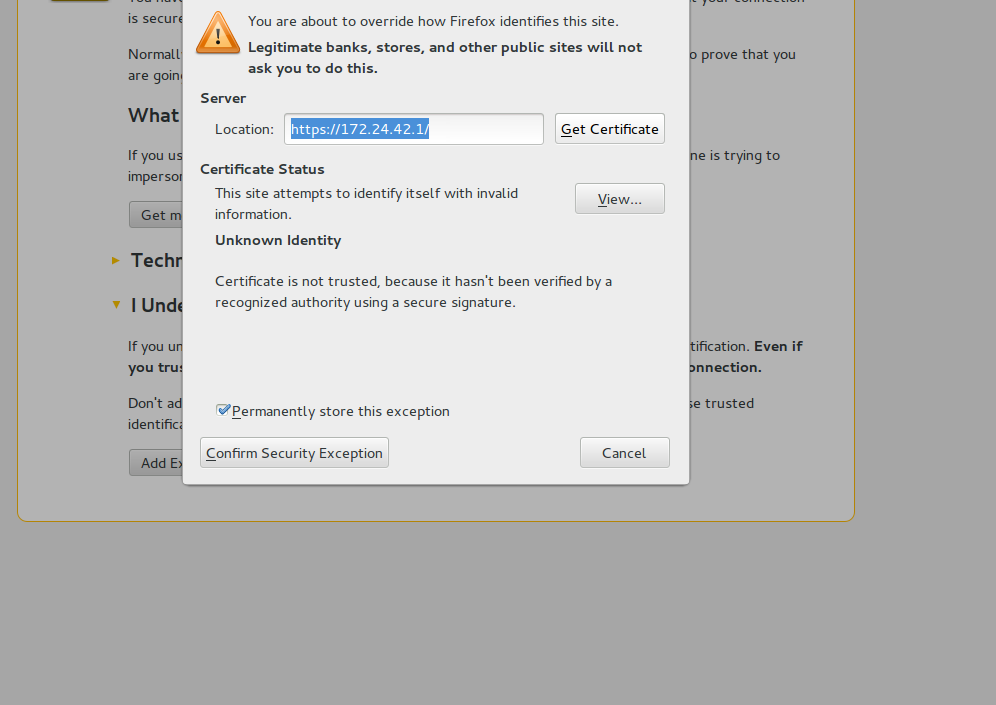
\includegraphics[width=0.70\textwidth]{ssl3.png}
  \end{center}
  \caption{Click: Get certificate and confirm}
\end{wrapfigure}



\begin{wrapfigure}{r}{1.00\textwidth}
  \begin{center}
    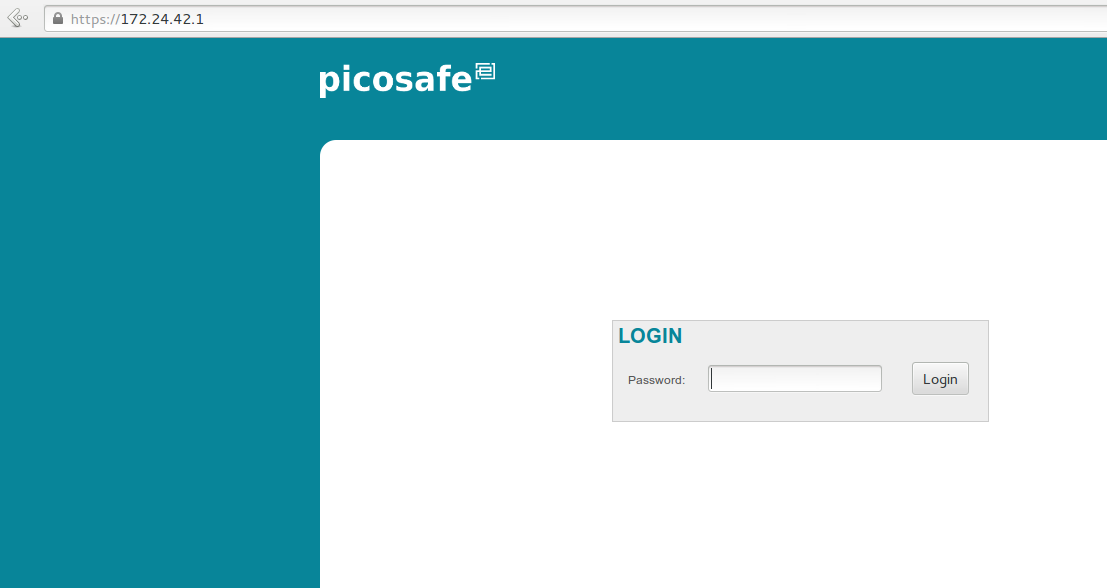
\includegraphics[width=0.60\textwidth]{picosafe_volumes_password.png}
  \end{center}
  \caption{Type your disk password (default: picosafe)}
\end{wrapfigure}

\begin{wrapfigure}{r}{1.0\textwidth}
  \begin{center}
    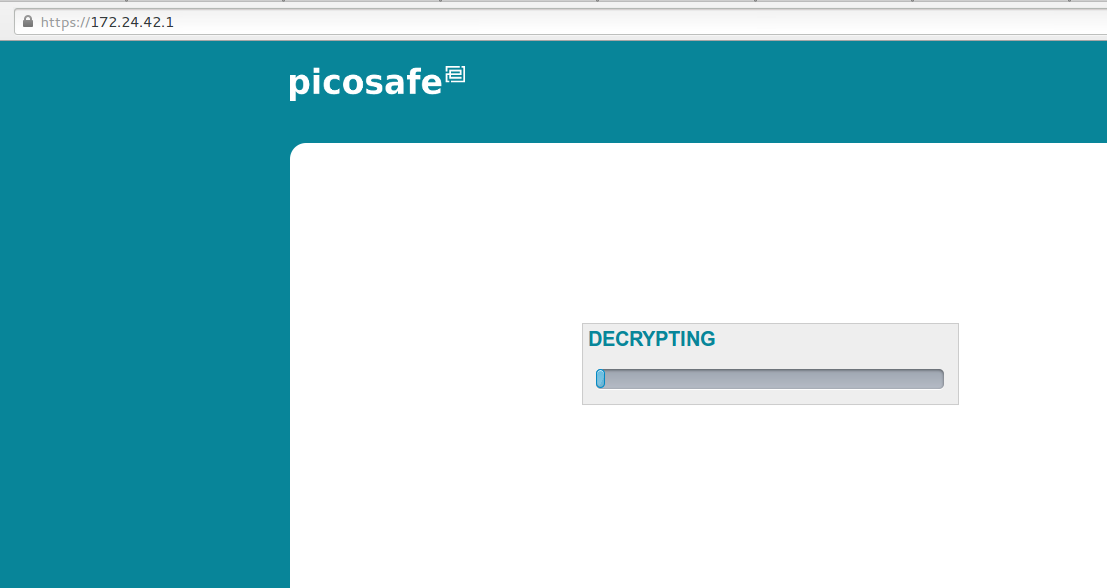
\includegraphics[width=0.60\textwidth]{picosafe_volumes_decrypting.png}
  \end{center}
  \caption{Wait while disk is decrypting}
\end{wrapfigure}

\begin{wrapfigure}{r}{1.0\textwidth}
  \begin{center}
    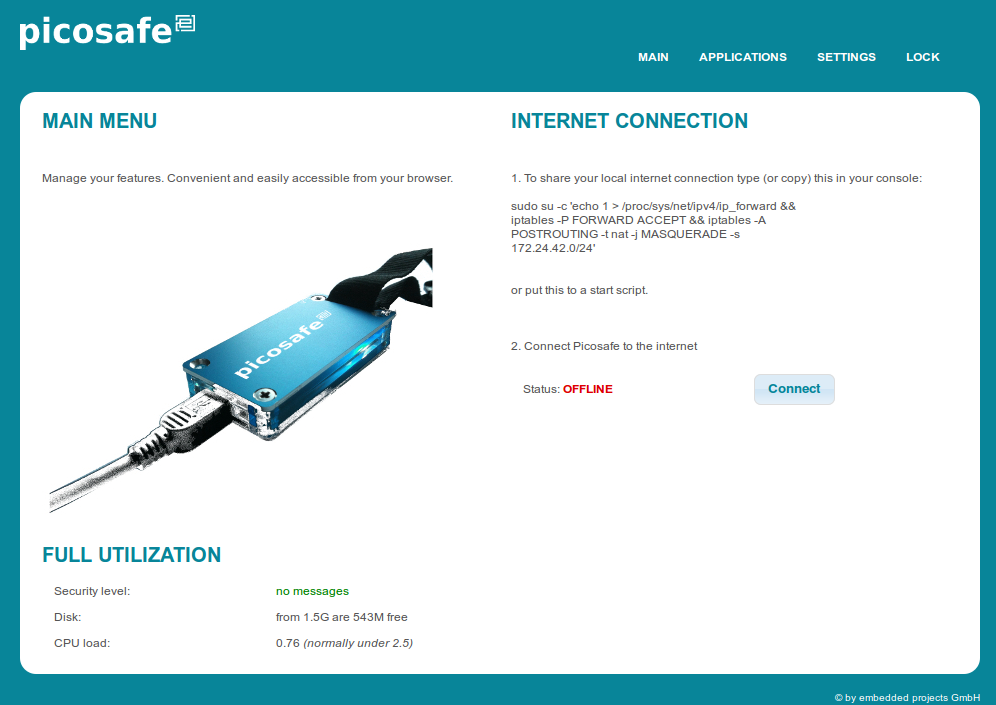
\includegraphics[width=0.60\textwidth]{picosafe_main.png}
  \end{center}
  \caption{Welcome screen on picosafe}
\end{wrapfigure}

\begin{wrapfigure}{r}{1.0\textwidth}
  \begin{center}
    
\includegraphics[width=0.60\textwidth]{white.png}
  \end{center}
\end{wrapfigure}

\chapter{Personalize and work with Picosafe}

\section{Connect with ssh}

Now you can connect you with ssh.


User: \texttt{picosafe} \\
Password: \texttt{picosafe} \\

Start ssh connection:

\texttt{ssh picosafe@172.24.42.1} \\

Change password:
\texttt{passwd} \\


\section{Change boot password for cryptsetup}

Default password: picosafe

You have to login via ssh and then type this commands:

\begin{itemize}

\item Show LUKS keys: \\
\texttt{sudo cryptsetup luksDump /dev/mmcblk0p3}

Tip: You have to type first your user password for picosafe (for sudo),
the your old boot password and the two times the new password for boot.


Now you can add a new password:


\item Add a LUKS key: \\
\texttt{sudo cryptsetup luksAddKey /dev/mmcblk0p3}


And remove the old picosafe password:

\item Remove LUKS key: \\
\texttt{sudo cryptsetup luksKillSlot /dev/mmcblk0p3 0}

\end{itemize}

\section{Set system clock}

You can setup system clock with the web gui in menu settings, 
or with commandline tools like

\texttt{sudo hwclock --set --date "2012/11/12 11:11:11"}

and

\texttt{sudo hwclock --hctosys}

or online 

\texttt{sudo rdate time.fu-berlin.de}

and then sync to hw clock
\texttt{sudo hwclock --systohc}

\section{Internet access with Linux Host}

To access internet from picosafe, perform on your host (as root) this command:

\texttt{su -c 'echo 1 > /proc/sys/net/ipv4/ip\_forward \&\& iptables -P FORWARD ACCEPT \&\& iptables -A POSTROUTING -t nat -j MASQUERADE -s 172.24.42.0/24'}

And click on the welcome main gui on connect.

\section{Internet access with Windows}

\section{Internet access with MacOS}

\section{Shutdown Picosafe}
\begin{itemize}
\item Disconnect
\item After the automatic shutdown time (in window settings) picosafe switched of automatic
\item There are two phase of shutdown
\item 1. Phase LED blinks as heartbeat: That means in about 10 seconds shutdown starts
\item If you will stop shutdown re-connect it fast to usb
\item 2. Phase LED blinks constant: Shutdown is running
\end{itemize}



\section{SSH Keys for further use}

Picosafe is really just a completely encrypted mini server from which you can very easily but securely connect to other SSH server itself. This surface is actually more of a help, because SSH is used for Picosafe with all original tools on the command line. 

With picosafe your private key never leaves the secure picosafe enviroment.

SSH tools on picosafe:

\begin{itemize}
\item ssh-key-gen to generate a key pair
\item ssh to start ssh connections
\item scp to copy files
\item ssh-copy-id to copy your public key to another server or pc
\item ssh-agent to remember during a session your passphrase
\end{itemize}

1. Generate first time a key pair (optional with a password)

\texttt{ssh-key-gen}

Additional you can protect you key pair with an passwort or so called passphrase. This means you can use the files only if you know the passpharse. 

2. Add external ssh servers to your SSH config
 
This means you don't have to type every time ssh user@domain.de. You can put the host, user, port and so on into an config file. Then you can define a short label. After this you can start a session with ssh yourlabel. That's it. 

You can do this with the web gui or directly over command line.

\begin{lstlisting}
Host yourlabel
  User username_on_server
  HostName domain_or_ip
  Post port_on_server 

\end{lstlisting}

Further hosts you can put also into this file.

3. Copy you public key to forgein servers

If you don't like to be ask every time you log into an server you can copy your public key on the external server. Then the server can this to authentifcate you.

\texttt{ssh-copy-id user@domain-or-ip}

or you can use your label from SSH config:

\texttt{ssh-copy-id yourlabel}

Now you have to write the last time the password. After this success you can login without a password. 

4. Work with ssh-agent or remember the password for your private key during a session

If you use an password or passphrase at you keys you need every time you use the keys this password or passphrase. ssh-agent is small tool which can start an session for example for two hours. That means in this time you don't need your password or passphrase again. Before you start to work type once:

\texttt{exec ssh-agent bash}

Then put your keys into the hand of the agent:

\texttt{ssh-add}

And start to work with you ssh accounts. 

5. Login to server behind servers

Sometimes a server is behind an central login server. This means you keys must be forward to the final server. You can enable this freature in you SSH config.

\texttt{ForwardAgent yes}

If you want to connect to a computer that is behind another, usually you have to shimmy through successively via SSH to. In the SSH config you can do this, however, define once and connect to a short machin1 ssh directly to the correct server behind other servers.


\begin{lstlisting}
Host machine1
  User username
  HostName domain-or-ip-rechner1

Host machine2
  User otherusername
  ProxyCommand ssh -q machine1 nc -q0 domain-or-ip-machine2 22
\end{lstlisting}

If one wants to also now not every log times with the password you can directly with its public key on machine2.

\texttt{ssh-copy-id machine2}


\section{Rescue Backup}


We recommend to do the first time a complete backup (dump) of your sd card.

After put your sd card into an pc (with an reader) find out what
device char you get.

\texttt{dmesg}

Then umount all partitions.

\texttt{sudo umount /dev/sdX1}

\texttt{sudo umount /dev/sdX2}

\texttt{sudo umount /dev/sdX3}

\texttt{sudo umount /dev/sdX4}

And final copy the complete image:

\texttt{sudo dd if=/dev/sdX of=picosafe\_backup\_image.bin}


You can recover the content to a new card with this command:

\texttt{sudo dd if=picosafe\_backup\_image.bin of=/dev/sdX}

You have to change also X with the correct char.




\section{Update}


Login with ssh (as picosafe). Then change the foler:


\texttt{cd /opt/picosafe}

And update with git:

\texttt{git pull}


Sometimes an SSL certificate error occours. This themes to be a bug of the git version. A quick fix is to export a variable:

\texttt{export GIT\_SSL\_NO\_VERIFY=1}

Then do the first pull

\texttt{git pull}

And now enable ssl verify again.

\texttt{export GIT\_SSL\_NO\_VERIFY=0}

At this time now you should be able to pull without this fix.
